\chapter{Java Orientado a Objetos G4 - ONE}
Porqu\'e aprender Java, es un lenguaje orientado a objetos, multiplataforma
la principal ventaja es la plataforma y esto nos va ayudar a tener un conjunto mayor de oportunidades,
La plataforma Java, seria la maquina virtual de Java, los frameworks, y la facilidad de impletar todos ellos.

Principales caracteristicas
\begin{itemize}
    \item Portable
    \item F\'acil de implementar
    \item Seguridad
    \item Omnipresente
\end{itemize}

La maquina virtual est\'a en bancos, dispositivos, computadores, la maquina virutal de java 

C\'odigo (Lenguaje Java) $\to$ Ejecutable (Bytecode) $\to$ Java Virtual Machine (JVM) $\to$ \{ Linux, Windows, Mac \}

Por ejemplo C\'odigo en Java: 
\begin{verbatim}
    package com.alura.Java
    public class Persona {
        String nombre;
        String apellido;
        int edad;

        void datosDefault(){
            this.nombre = "Diego";
            this.apellido = "Arguelles";
            this.edad = 28;
        }
    }
\end{verbatim}

Bytecode

\begin{figure}[h!]
    \center
    \begin{minipage}{5cm}
    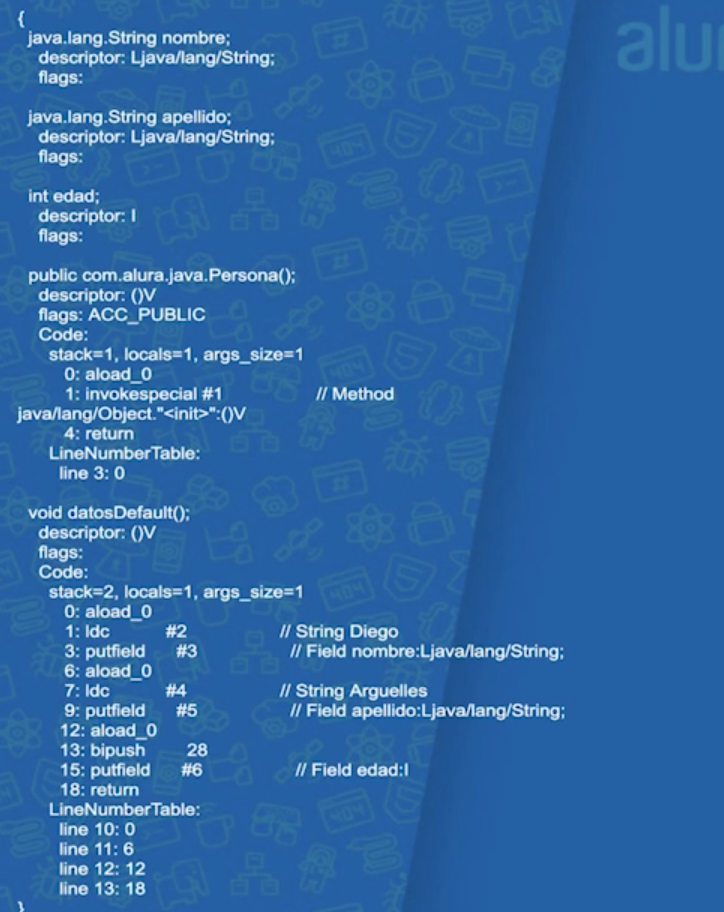
\includegraphics[width=4cm]{Develop/Languages/Java/images/Captura desde 2023-02-07 23-21-16.png}
    \end{minipage}
  \end{figure}

Este lenguaje en la imagen es el que interpreta la JVM, ?`La JVM solo compila c\'odigo? Est\'a tambi\'en se 
encarga de 
\begin{itemize}
    \item Administraci\'on de memor\'ia. 
    \item Multiplataforma.
    \item Seguridad.
    \item Optimizaci\'on.
    \item Librer\'ias.
\end{itemize}

los siguientes lenguajes son soportados en la maquina virtual de Java, 
Ruby, Scala, python, cljs, Grooby y a su vez la JVM es soportada por MAC, Windows y Linux.

?` Cu\'al es la diferencia entre archivos ejecutables de Windows (.exe) y archivos ejecutables de Java (Bytecode)?:

Los ejecutables de Windows pueden correr directamente en el sistema operativo, los de java necesitan de la maquina virtual. 

Los archivos ejecutables de Java son port\'atiles, los de windows no.


\section{Copilando mi primer Hola mundo}

\begin{verbatim}
    public class  HolaMundo {
        public static void main(String[] args){
            System.out.println("Hola mundo");
        }
    }
\end{verbatim}


Al ejecutar el IDE de eclipse me sale el siguiente error

\begin{verbatim}
Picked up _JAVA_OPTIONS: -Dawt.useSystemAAFontSettings=on -Dswing.aatext=true

Error occurred during initialization of boot layer

java.lang.module.FindException: 
Error reading module: /home/kali/eclipse-workspace/SintaxeBasica/bin

Caused by: 
java.lang.module.InvalidModuleDescriptorException: 
Programa.class found in top-level directory (unnamed package not allowed in module)
\end{verbatim}

lo he solucionado eliminado el archivo module-info.java


\section{Data types}
Data types are divided into two groups: 
\begin{itemize}
    \item Primitive data types - includes {\red byte, short, int long, float, double, boolean and char}.
    \item Non-primitive data types - such as {\red String, arrays and classes }
\end{itemize}

\subsection{Primitive Data Types}
A primitive data type specifies the size and type of variable values, and it has no additional methods. There are eight primitive data types in Java: 
\begin{center}
\begin{tabular}[b]{l l m{12cm}}
\textsf{Data Type}  &  \textsf{Size} 	  &  \textsf{Description}                                                                          \\ \hline      
{\red byte} 	    & 1 byte   & Stores whole numbers from -128 to 127                                                \\ \hline                                
{\red short} 	    & 2 bytes  & Stores whole numbers from -32,768 to 32,767                                          \\ \hline                                      
{\red int} 	        & 4 bytes  & Stores whole numbers from -2,147,483,648 to 2,147,483,647                            \\ \hline                                                    
{\red long} 	    & 8 bytes  & Stores whole numbers from -9,223,372,036,854,775,808 to 9,223,372,036,854,775,807    \\ \hline                                                                            
{\red float} 	    & 4 bytes  & Stores fractional numbers. Sufficient for storing 6 to 7 decimal digits              \\ \hline                                                                  
{\red double} 	    & 8 bytes  & Stores fractional numbers. Sufficient for storing 15 decimal digits                  \\ \hline                                                              
{\red boolean}      & 1 bit 	  & Stores true or false values                                                          \\ \hline                      
{\red char} 	    & 2 bytes  & Stores a single character/letter or ASCII values                                     \\ \hline                                           
\end{tabular}
\end{center}

declaring some primitive values except for Strings what is a object of Java:  

\begin{verbatim}
public class Main {
    public static void main(String[] args) {
      int a = 24;
      double x = 4.5;
      long y = 456321;
      boolean yes = true;
      char a = 'A'; // hace refencia a los valores de https://www.asciitable.com/
      String myText = "Hello";
    }
  }  
  
  
public class Main {
    public static void main(String[] args) {
      int myNum = 5;               // integer (whole number)
      float myFloatNum = 5.99f;    // floating point number
      char myLetter = 65;    		// character
      char myLetterPlusOne =  (char) (myLetter +1);
      boolean myBool = true;       // boolean
      String myText = "Hello ";     // String    
      System.out.println(myNum);
      System.out.println(myFloatNum);
      System.out.println("myLetterPlusOne " + myLetterPlusOne);
      System.out.println(myBool);
      System.out.println(myText + myNum);
    }
}   
\end{verbatim}
Las variables en Java guardan valores y no direcciones ni punteros.


Non-Primitive Data Types

Non-primitive data types are called reference types because they refer to objects.

The main difference between primitive and non-primitive data types are:
\begin{itemize}
    \item Primitive types are predefined (already defined) in Java. Non-primitive types are created by the programmer and is not defined by Java (except for String).
    \item Non-primitive types can be used to call methods to perform certain operations, while primitive types cannot.
    \item A primitive type has always a value, while non-primitive types can be null.
    \item A primitive type starts with a lowercase letter, while non-primitive types starts with an uppercase letter.
    \item The size of a primitive type depends on the data type, while non-primitive types have all the same size.
\end{itemize}
Examples of non-primitive types are Strings, Arrays, Classes, Interface, etc. You will learn more about these in a later chapter.

\section{Type Casting}

Type casting is when you assign a value of one primitive data type to another type.

In Java, there are two types of casting:

\begin{itemize}
    \item Widening Casting (automatically) - converting a smaller type to a larger type size
    \begin{center}
    byte $\to$ short $\to$ char $\to$ int $\to$ long $\to$ float $\to$ double
    \end{center}
    \item Narrowing Casting (manually) - converting a larger type$ to$ a smaller size type
    \begin{center}
        double $\to$ float $\to$ long $\to$ int $\to$ char $\to$ short $\to$ byte 
    \end{center}
\end{itemize}

\subsection{Widening Casting}
Widening casting is done automatically when passing a smaller size type to a larger size type:

\begin{verbatim}
public class Main {
  public static void main(String[] args) {
    int myInt = 9;
    double myDouble = myInt; // Automatic casting: int to double

    System.out.println(myInt);      // Outputs 9
    System.out.println(myDouble);   // Outputs 9.0
  }
}
\end{verbatim}

\subsection{Narrowing Casting}

Narrowing casting must be done manually by placing the type in parentheses in front of the value: 

\begin{verbatim}
    public class Main {
        public static void main(String[] args) {
          double myDouble = 9.78d;
          int myInt = (int) myDouble; // Manual casting: double to int
      
          System.out.println(myDouble);   // Outputs 9.78
          System.out.println(myInt);      // Outputs 9
        }
      }      
\end{verbatim}

\section{Operators}


Operators ara used to perform operations on variables and values.

In the exxample below, we use the $+$ operator to add together two values: 

\begin{verbatim}
  int x = 100 + 50;
\end{verbatim}

Java divides the operators into the following groups: 

\begin{itemize}
  \item Arithmetic operators 
  \item Assignment operators
  \item Comparasion operators
  \item Logical operators
  \item Bitwise operators
\end{itemize}

\subsection{Arithmetic Operators}

Arithmetic operators are used to perform common mathematical operations.

\begin{center}
\begin{tabular}[t]{l l l l}
  {\bf Operator} & {\bf Name}     & {\bf Description}                    & {\bf Example} \\
       $+$       & Addtion        & Adds together two values             & $x+y$ \\
       $-$       & Multiplication & Multiples two values                 & $x*y$ \\
       $*$       & Division       & Divides one value by another         & $x/y$ \\
       $\%$      & Modulus        & Return the division remainder        & $x\% y$ \\
       $++$      & Increment      & Increases the value of variable by 1 & $++x$ \\
       $--$      & Decrement      & Decreases the value of variable by 1 & $--x$ \\
\end{tabular}
\end{center}

\subsection{Assignment Operators}

Assignment operators are used to assign values yo variables.

In the example below, we use the assignment operator $(=)$ to assign the value 10 to variable called {\bf x}: 

\begin{verbatim}
  int x = 10;
\end{verbatim}

The addition assignment operator $(+=)$ adds a value to a variable: 


\section{Strings}

Strings are used for storing text. 

A string variable contains a collection of characters surrounded by double quotes: 

\begin{verbatim}
  String greeting = "Helllo";
\end{verbatim}

String Length: A String in Java is actually an object, which contain methods that can perform certain operations on strings. 
For example, the length of a string can be found with the length() method: 

\begin{verbatim}
public class Main {
  public static void main(String[] args) {
    String txt = "ABCDEFGHIJKLMNOPQRSTUVWXYZ";
    System.out.println("The length of the txt string is: " + txt.length());
  }
}
\end{verbatim}

More String Methods: there are many methods avalaible, for example toUpperCase() and toLowerCase(): 

\begin{verbatim}
  public class Main {
    public static void main(String[] args) {
      String txt = "Hello World";
      System.out.println(txt.toUpperCase());
      System.out.println(txt.toLowerCase());
    }
  }  
\end{verbatim}

\subsection{Finding a Character in a String}

The indexOf() method returns the index (the position) of the first occurrence of specified text in a string (including whitespace): 

\begin{verbatim}
public class Main {
    public static void main(String[] args) {
      String txt = "Please locate where 'locate' occurs!";
      System.out.println(txt.indexOf("locate"));
    }
}  
\end{verbatim}

\subsection{Complete String Reference}

For a complete reference of String methods, go to our \href{https://www.w3schools.com/java/java_ref_string.asp}{Java String Methods Reference}. 

\subsection{Special Characters}

Strings - Special Characters

Because strings must be written within quotes, java will misunderstand this string, and generate an error: 

\begin{verbatim}
String txt = "We are the so-called "Vikings" from the north.";
\end{verbatim}

The solution to avoid this problem, is to use the backslash escape character.

The backslash $(\backslash)$ escape character turns special characters into string characters: 
\begin{center}
\begin{tabular}[t]{l l l}
         {\bf Escape charater}   & {\bf Result}   & {\bf  Description} \\
         $\backslash '$          &     '        & Single quote        \\
         $\backslash \backslash$  & $ \backslash$  & Backslash  \\
\end{tabular}
\end{center}

The sequence $\backslash" $ inserts a double quote n a string: 

\begin{verbatim}
public class Main {
  public static void main(String[] args) {
    String txt = "We are the so-called \"Vikings\" from the north.";
    System.out.println(txt);
  }
}
\end{verbatim}

the sequence $\backslash '$ inserts a single quote in a string: 

\begin{verbatim}
  public class Main {
    public static void main(String[] args) {
      String txt = "It\'s alright.";
      System.out.println(txt);
    }
  }  
\end{verbatim}

Other common escape sequences that are valid in Java are:

\begin{center}
  \begin{tabular}[t]{ l l}
    Code  &  	Result                         \\ \hline
    $\backslash$n 	  & New Line 	           \\  
    $\backslash$r 	  & Carriage Return 	   \\  
    $\backslash$t 	  & Tab 	               \\   
    $\backslash$b 	  & Backspace 	         \\  
    $\backslash$f 	  & Form Feed            \\  \hline
  \end{tabular}
\end{center}


\subsection{Java Booleans}

Very often,  

\section{Methods}

A method is a block of code which only runs when it is called.

You can pass data, known as parameters, into a method.

Methods are used to perform certaon actions, and thet are also known as functions. 

Why use methods? To reuse code: define the code once, and use it many times. 

Create a Method

A method must be declared within a class. It is defined with the name of the method, followed by parentheses (). Java provides some pre-defined methods, such as System.out.println(), but you can also create your own methods to perform certain actions:

\begin{verbatim}
Example

Create a method inside Main:

public class Main {
  static void myMethod() {
    // code to be executed
  }
}
\end{verbatim}

Example Explained
\begin{description}
  \item[myMethod(): ] is the name of the method.
  \item[static: ] means that the method belongs to the Main class and not an object of the Main class. You will learn more about objects and how to access methods through objects later in this tutorial.
  \item[void: ] means that this method does not have a return value. You will learn more about return values later in this chapter
\end{description}
    
Call a method 

To call a method in JAva, write the method's name followed by two parentheses () and a semicolon; In the following example. myMethod() is 
used to print a text (the action), when it is called: 

\begin{verbatim}
  Inside main, call the myMethod() method:

  public class Main {
    static void myMethod() {
      System.out.println("I just got executed!");
    }
  
    public static void main(String[] args) {
      myMethod();
    }
  }
  
  // Outputs "I just got executed!"
\end{verbatim}
    

\chapter{Java OO: entendiendo la orientaci\'on a objetos}

?`Qu\'e ventajas tiene conocer orientaci\'on a objetos?

Alta cohesi\'on bajo acoplamiento. comprender conceptos b\'asicos de encapsulamiento, 
creaci\'on de c\'odigo reutilizable. Ampliamente utilizado por la mayor\'ia de lenguajes de programaci\'on .
T\'ecnicas para consumir c\'odigo creado en otras librer\'ias.


Proyecto de entidad finaciera llamada  by bank, tendra tidos de entidades, los clientes, cuentas, tendra comportamientos y 
operaciones, estos son comportamientos que son anexados a la entidad cuenta. 

Definamos el conjunto de caracteristicas que tendra nuestra cuenta, tendr\'a cuatro campos 

\begin{center}
  \begin{tabular}[t]{l l}
    Campo       &     Value\\ \hline
    saldo 	    &   	     \\  
    agencia 	  &   	     \\  
    numero 	    &  	       \\   
    titular 	  &  	       \\ \hline
  \end{tabular}
\end{center}

\section{Herencia e interfaces}
